\chapter{正演数据处理}
 正演地震数据直接进行抽道集和速度分析,进行叠加,没有去除噪音这一个步骤。搞清楚“common-depth-point” (CDP)  and  “common midpoint” (CMP) 两个概念的差异
 \section{定义观测系统}
用 suchw 创建道头cdp 并赋值,通过gx (key2) and sx (key3)两个来计算(与sushw不同)
\begin{lstlisting}
key1 = ( a + b*key2 + c*key3 ) / d
\end{lstlisting}
a,b,c通过观测系统确定,例如 a = 1525, b =1, c = 1, and d = 50.
\begin{lstlisting}
cdp = ( 1525 + 1*gx + 1*sx ) / 50
suchw < seis4.su key1=cdp key2=gx key3=sx a=1525 b=1 c=1 d=50 >seishw.su
\end{lstlisting}

\section{抽道集}
利用susort抽道集基于第一关键字cdp和第二关键字offset。第二关键字是在第一关键字里面进行排序。
\begin{lstlisting}
 susort <seishw.su cdp offset> cmp4.su 
 susort <seishw.su > cmp4.su cdp offset
\end{lstlisting}
利用suwind、suxwigb、supswigb加入循环每隔多少个cdp进行显示查看剖面。关于覆盖次数的计算,有机会写一个小工具进行计算(pyqt)

\section{叠加速度分析}
速度有层速度、均方根速度、叠加速度、偏移速度。\par
\subsection{速度分析前的准备}
速度分析前的准备,常规地震处理(例如多次波、噪音的移除、直达波和折射波切除):
\begin{lstlisting}
sumute<data.su key=tracf  xmute=1,46,48 tmute=2.250,0.500,0.004 > $outdata
\end{lstlisting}
\subsection{suvelan进行速度分析}
通过cmp道集速度分析时,为了能够减少速度分析的时间需要人为设置速度分析的最小值和最大值。\par
suvelan 在每个时间都nmo正常时差校正并叠加,速度从 4000 到 12000 $(=(50*160)+4000 ) f/s$,增量为50$(dv)$。\par
suxcontour中nc参数是等值线级数控制。
\begin{lstlisting}
 indata=oz14h.su
 # Important processing variables
 # nv = number of vels, dv = delta vel, fv = first vel
 nv=160
 dv=50
 fv=4000
 # Do the work
 suvelan < $indata nv=$nv dv=$dv fv=$fv smute=1.5 |
 suxcontour bclip=0.5 wclip=0.0 f2=$fv d2=$dv label1=" Time (s)" label2="Velocity"  title="Semblance plot for CMP $indata" windowtitle="Semblance: $indata" grid1=solid grid2=solid cmap=default nc=7 nlabelc=0 
\end{lstlisting}

\subsection{常速度叠加}
常速度叠加  /  constant velocity stacks (CVS)
\begin{lstlisting}
#! /bin/sh
# File: migcvp.sh
#       Create one panel for each migration velocity
#       Each panel has the same "fldr" value
#       The migration velocity is in key "offset"
#       Total number of panels is in key "nvs"
indata=stack4.su    # SU format
outdata=migcvp.su   # migration Constant Velocity Panels

# Migration variables
cdpmin=80      # Start CDP value
cdpmax=150     # End CDP value
dxcdp=70.71    # distance between adjacent CDP bins (m)
smig=1.0       # stretch factor (0.6 typical if vrms increasing)
# [the "W" factor] (Default=1.0)
vscale=1.9     # scale factor to apply to velocities (Default=1.0)
lstaper=20     # length of side tapers (traces) (Default=0)
lbtaper=100    # length of bottom taper (samples) (Default=0)

# Velocity panel variables
firstv=1200    # first velocity value
lastv=5000    # last velocity value
increment=200  # velocity increment

numVtest=100   # use to limit number of velocity panels
# otherwise, use very large value (100)
# Compute number of velocity panels
numV=`bc -l << -END
( ( $lastv - $firstv ) / $increment ) + 1
END`

if [ $numVtest -lt $numV ] ; then
numV=$numVtest
fi
# FILE DESCRIPTIONS
# tmp1 = binary temp file of input data
cp $indata tmp1
migV=$firstv
#-------------------------------------
# Loop through Migration Constant Velocity Panels
#     Each panel has the same "fldr" value
#     Panel migration velocity is in key "offset"
#     Total number of panels (numV) is in key "nvs"
#-------------------------------------
i=1
while [ $i -le $numV ]
do
suwind < tmp1 key=cdp min=$cdpmin max=$cdpmax |sushw key=fldr a=$i |sushw key=offset a=$migV |sushw key=nvs a=$numV |
sustolt cdpmin=$cdpmin cdpmax=$cdpmax dxcdp=$dxcdp tmig=0 vmig=$migV smig=$smig vscale=$vscale lstaper=$lstaper lbtaper=$lbtaper >> $outdata

i=`expr $i + 1`
migV=`expr $migV + $increment`
done
rm -f tmp*
\end{lstlisting}
常速度偏移剖面放映
\begin{lstlisting}
indata=migcvp.su
perc=98
loop=1       # run panels forward continuously
# 2 = run panels back and forth continuously
# 0 = load all panels then stop
n1=501       # number of time samples
d1=0.004     # time sample interval
n2=71        # number of traces per panel
d2=1         # trace spacing
width=300    # width of window
height=500   # height of window
fframe=1200  # velocity of first panel for title annotation
dframe=200   # panel velocity increment for title annotation
suxmovie < $indata perc=$perc loop=$loop n1=$n1 d1=$d1 n2=$n2 d2=$d2  width=$width height=$height fframe=$fframe dframe=$dframe title="Velocity %g" 
\end{lstlisting}
\subsection{速度分析质量控制}
\begin{enumerate}
	\item a graph of the velocity profile;	速度剖面显示
	\item a plot of the NMO-corrected CMP;	cmp拉平之后显示
	\item a plot of the stack trace repeated eight times;	叠加剖面
	\item 之前拾取的速度也应该显示在剖面上便于下次拾取
	\item 地震剖面中隔几个cmp进行速度分析一次取决于地质结构的复杂程度
	\item 速度分析见附件iva.sh
\end{enumerate}\par
速度库质量控制tvnmoqc model=1速度库文件检查(拾取的速度不是递增能检查出来),mode=2两种模式,具体见附件v-tcheck.sh和velanQC.sh。对出现问题的速度库进行重新拾取。
\section{正常市场校正、叠加}
\subsection{正常时常校正,sunmo}
\begin{lstlisting}
sunmo < $indata cdp=60,80 tnmo=0.0158311,0.390501,0.686016,1.06069,1.99472vnmo=1511.85,1511.85,2640.45,2922.6,3249.3 tnmo=0.0158311,0.353562,0.701847,1.0343,1.99472 vnmo=1482.15,1511.85,2625.6,2774.1,2982 > outdata.s
\end{lstlisting}\par
CMP之间的速度是通过插值得到的,有时候差值会起到反效果,需要进行加密\par
查看校正之后的结果,见脚本iview.sh
\subsection{叠加,sustack}
\begin{lstlisting}
sustack < nmo4a.su > stack4.su
\end{lstlisting}\par
默认的关键字key为cdp,所以可以省略

\section{偏移}
\begin{lstlisting}
time=0.00,0.70,0.75,0.80,0.85,0.90,2.00
vels=1500,1500,2500,3000,2800,3100,3500

sustolt < stack4.su cdpmin=1 cdpmax=458 dxcdp=70.71 tmig=$time vmig=$vels smig=0.6 vscale=1.9 lstaper=20 lbtaper=100 | 
\end{lstlisting}
sustlot(偏移速度快)参数:\\
\begin{tabular}{lllp{0.55\textwidth}}
	\toprule
	Name  & optional &Default &  Descrption\\
	\midrule
	cdpmin & R & & minimum CDP number for which to apply DMO\\
	cdpmax &  R &  &  maximum CDP number for which to apply DMO\\
	dxcdp  &  R &  &  distance between adjacent CDP bins (m)\\
	noffmix & O & 1 & number of offsets to mix (for unstacked data only)\\
	tmig & O & 0.0 & times corresponding to RMS velocities in vmig (s)\\
	vmig & O & 1500. & RMS velocities corresponding to times in tmig (m/s)\\
	smig  & O & 1.0 & stretch factor (0.6 typical if Vrms increasing)\\
	vscale & O & 1.0 & scale factor to apply to all velocities  \\  	
	fmax & O & & Nyquist maximum frequency in input data (Hz)\\
	lstaper & O & 0 & length of side tapers (traces)\\
	lbtaper &  O & 0  & length of bottom taper (samples)\\
	\bottomrule
\end{tabular}\par
cdpmin和cdpmax是必须的参数,是指定特定的cdp范围实施DMO,但是通常我们包括所用的cdp点。换而言之在使用sustlot算法之前通常都是先使用DMO校正(dip moveout correction)\par
dxcdp参数为CDP bin距离:(Thediagonal line of Common Midpoint Direction cuts the diagonal of 50 meter x 50 meterboxes.)\par
Common Midpoint Distance = sqrt( 50x50 + 50x50 ) = 70.71 m\par
设置伸长因子,参数smig:常速度偏移为1.0,随时间变化设置为0.6\par
设置fmax值小于nyquist频率能够减少运算量\par
lstaper=20和lbtaper=100为边界和底部逐渐减少的值,需要实验。\par
偏移能够得到地下的结构的速度,能够使地下介质正确归位的速度,看成是层状介质的均方根速度。\par
图\ref{fig:sustlot}左边为stolt偏移之后结果,由于速度分析做的不精确,速度跳变的地方出现画弧现象。\\
\begin{figure}[htbp]
	\centering
	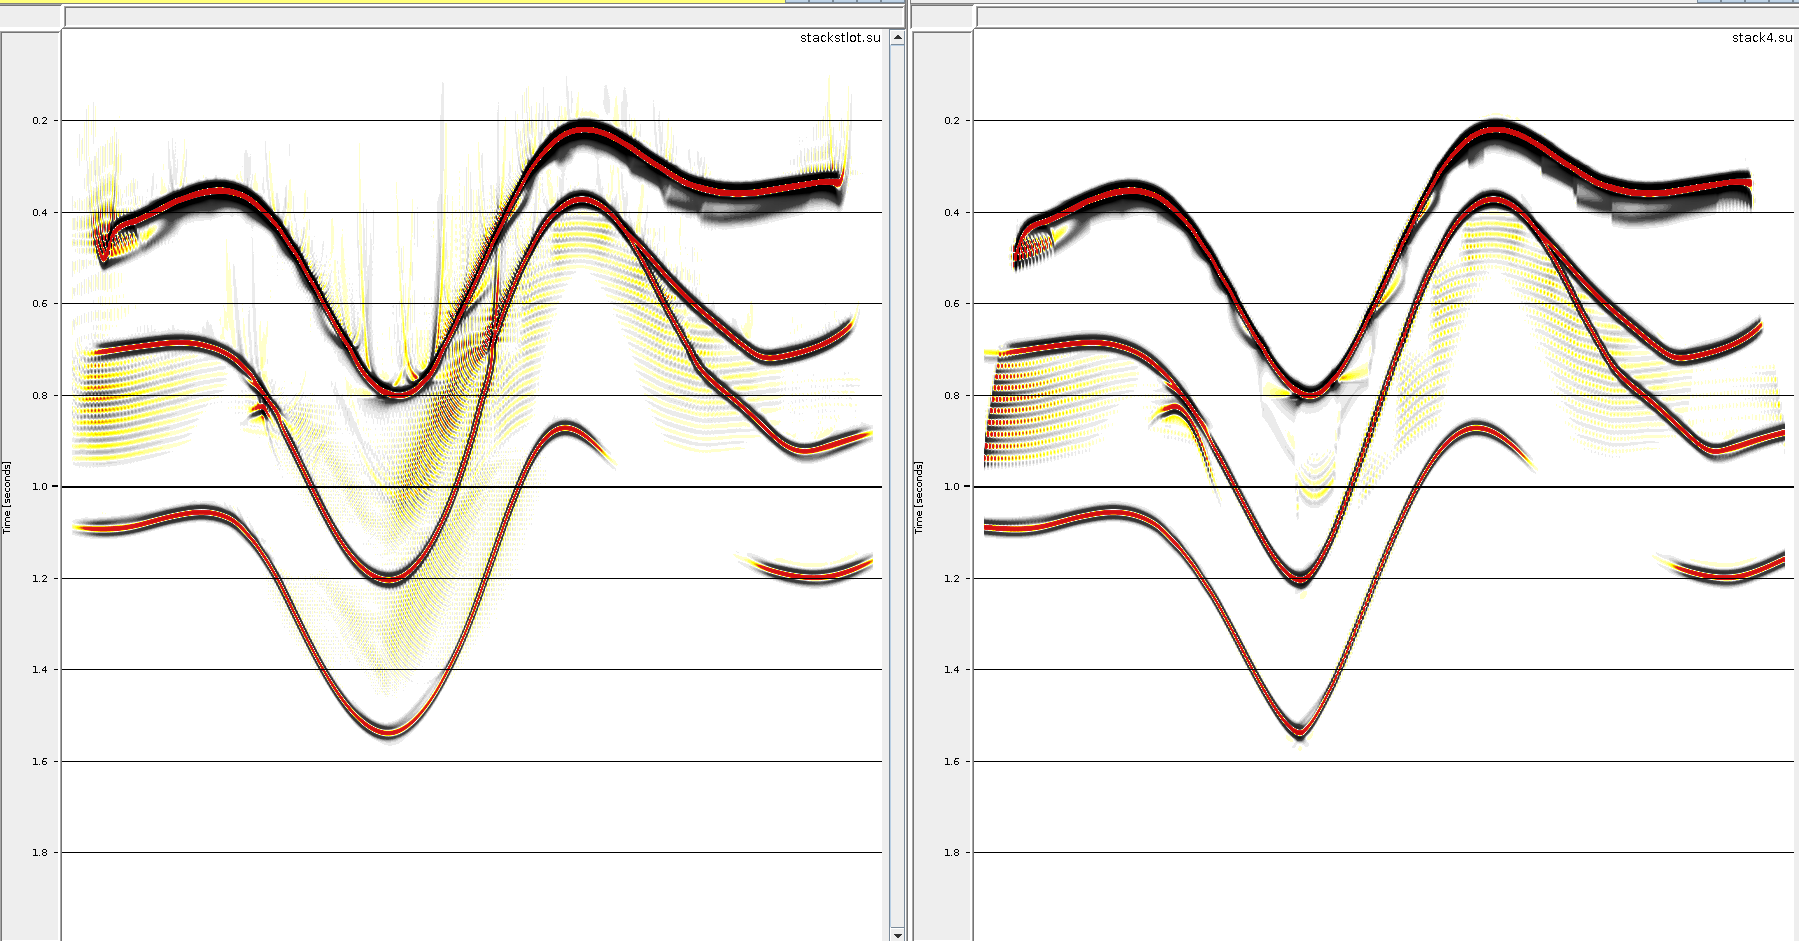
\includegraphics[bb=0 0 1295 678,scale=.25]{SU/fig/stoltmig.png}
	\caption{sustlot偏移}
	\label{fig:sustlot}
\end{figure}
